%% !TEX root = ../main.tex
\chapter{La Composition de services web}
\label{ch:composition}

\section*{Introduction}
\addcontentsline{toc}{section}{Introduction} \markboth{INTRODUCTION}{}

Dans le chapitre précédent \ref{ch:web-service}, nous avons présenté
la description, la publication et la découverte des services Web où une
requête d'un utilisateur peut être satisfaite par l'invocation d'un
seul service Web référencé dans un annuaire. Si l'objectif du client
n'est pas atteint par l'invocation d'un simple service Web
élémentaire, alors il doit combiner les fonctionnalités d'un ensemble
de services afin d'accomplir l'objectif désiré. Ce processus est
appelé \textit{``composition des services Web''}. Le problème de la
composition des services Web se réfère à la construction des nouveaux
services Web à plus forte valeur ajoutée \textit{``services
  composites''} à partir des services individuels existants
\textit{``services atomiques''}.\bigskip

Dans ce chapitre, nous allons présenter les travaux liés à la
composition des services Web qui constitue le cœur de notre
problématique. Nous présentons dans un premier temps les définitions
et les stratégies de composition des services Web présentes dans la
littérature \ref{sec:defs}, puis nous étudions quatre langages majeurs
de composition des services \ref{sec:lang-de-comp}. Ensuite, nous
allons décrire et classifier les différentes approches de composition
dynamique proposées par la littérature \ref{sec:comp-dynam}. La dernière 
section \ref{sec:graph-base-composition} sera
consacrée à analyser les techniques de composition basées sur le modèle
\textit{graphe} pour représenter les dépendances fonctionnelles entre
les services Web.

\newpage
\section{Définitions et stratégies de composition}
\label{sec:defs}
Cette section a pour but d'exposer, d'une part, quelques définitions
et objectifs de la composition de services Web proposées par la
communauté \ref{sec:definitions}, et d'autre part, les différents
types et mécanismes de composition selon différents points de vue
rencontrés dans la littérature \ref{sec:proc-de-coord},
\ref{sec:types-de-composition}.

  \subsection{Définitions}
  \label{sec:definitions}
  Martin \emph{et al.} \cite{martin2004owl} définissent la composition
  comme étant \emph{``le processus de sélection, de combinaison et
    d'exécution des services en vue d'accomplir un objectif
    donné''}.\bigskip

  Selon S. Dustdar et W. Schreiner \cite{dustdar2005survey} : \emph{``
    L'infrastructure de base des services Web suffit pour la mise en
    œuvre d'interactions simples entre un client et un service Web. Si
    la mise en œuvre d'une application métier implique l'invocation
    d'autres services web, il est nécessaire donc de combiner les
    fonctionnalités de plusieurs services web. Dans ce cas, nous
    parlons d'une composition de services Web''}.\bigskip

  En d'autre terme, La composition de services Web désigne une
  opération qui consiste à construire de nouvelles applications ou
  services appelés \textbf{services composites} ou agrégats par
  l'assemblage ou l'agrégation de services existants nommés
  \textbf{services atomiques} ou élémentaires.\bigskip

  Medjahed \cite{medjahed2004thesis} de ça part a défini un service
  Web composite comme un \emph{``conglomérat de sous-traitance
    services Web (services appelés participants) travaillant en tandem
    pour offrir un service à valeur ajoutée.''}\bigskip

  La composition des services Web vise essentiellement quatre objectifs
  \cite{driss2011approche}:

  \begin{enumerate}
  \item Créer de nouvelles fonctionnalités en combinant des services
    déjà existants.
  \item Résoudre des problèmes complexes auxquels aucune solution\\
    n'a été trouvée.
  \item collaborer plusieurs entreprises ensemble.
  \item Optimiser et améliorer une fonctionnalité existante.
  \end{enumerate}

  \subsection{Cycle de vie d'une composition }
  \label{sec:cycle-de-vie}
  Comme l'illustre la figure \ref{fig:composition-life-cycle}, le
  cycle de vie de la composition de services Web comprend quatre
  phases \cite{sheng2014web}: la phase de \textit{définition}, La
  phase de \textit{sélection}, la phase de \textit{déploiement} et la
  phase d'\textit{exécution}:

  \begin{figure}[h]
    \centering
    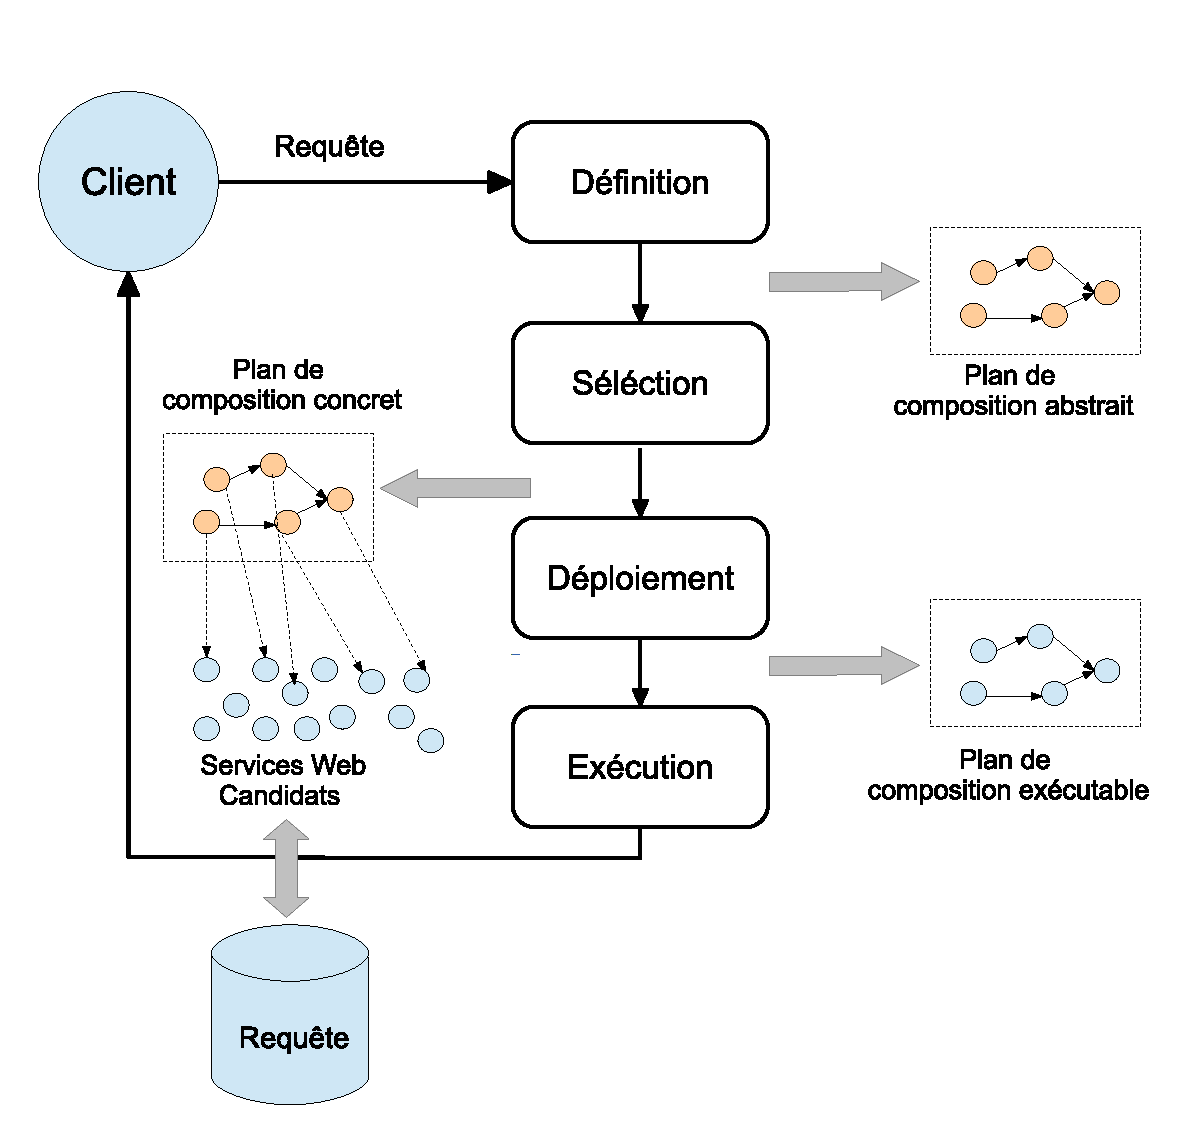
\includegraphics[width=0.9\textwidth]{figs/composition-life-cycle.eps}
    % TODO translate the figure
    % TODO reference the fig
    \caption{Cycle de vie d'une composition des services
      \cite{sheng2014web}.}
    \label{fig:composition-life-cycle.eps}
\end{figure}

%%% Local Variables:
%%% mode: latex
%%% TeX-master: "../main"
%%% End:


  \renewcommand{\descriptionlabel}[1]{\hspace{0.5cm}\textbullet~\textsf{#1}}
  \begin{description}
  \item[La phase de définition]: Pendant cette phase, le client de
    service spécifie les exigences de composition de services en termes
    des besoins et des préférences pour le service
    composite. l'exigence est ensuite \textit{décomposé}, soit
    semi-automatiquement ou automatiquement dans un modèle de
    \textbf{processus abstrait}(càd le service composite
    abstrait), qui spécifie l'ensemble d'activités, le contrôle,
    le flux de données entre eux, la qualité de service \acrshort{qos}
    , et la gestion des exceptions.

  \item[La phase de sélection]: Dans cette phase, pour chaque activité
    dans le service composite, les services Web appropriés qui
    répondent aux exigences de l'activité sont situés en cherchant dans
    le registre des services, sur la base des informations contenue
    dans les documents de description de service publiées. Il est
    probable que plus d'un service candidat peut répondre aux
    exigences. Par conséquent, le meilleur service identifié doit
    être sélectionné. Après tous, les services Web requis sont
    identifiés et liés aux activités correspondantes, le service
    composite construit est produit.

  \item[La phase de déploiement]: Dans cette phase, le service
    composite construit est déployé pour permettre son instantiation
    et l'invocation par les utilisateurs finaux. Le résultat de cette
    phase est le service composite exécutable.

  \item[La phase d'exécution]: Dans cette phase, l'instance de service
    composite est créée et exécutée par le moteur d'exécution, qui est
    aussi responsable de l'invocation des composants des service
    atomiques. Pendant l'exécution de l'instance du service composite,
    les tâches de surveillance, y compris le suivi d'exécution, la mesure
    de performance, et la gestion des exceptions, doivent être
    effectuées.
  \end{description}
  \enddescription

  \subsection{Procédés de coordination}
  \label{sec:proc-de-coord}
  Nous distinguons deux méthodes utilisées pour décrire la composition
  des services dans un flot de processus métier: l'\emph{orchestration}
   et la \emph{chorégraphie} des services. Ces deux
  procédés de coordination décrivent deux aspects de création des
  processus métiers à partir de services Web composites
  \cite{peltz2003web}.\medskip

  \textbf{Un procédé} est représenté par un graphe orienté d'activités
  ou un flot de contrôle qui donne l'ordre d'exécution des activités
  et la logique de coordination des services. Chaque activité
  représente une fonctionnalité réalisée concrètement par un service
  \cite{chollet2009orchestration}.\medskip

  Il convient de noter que ces modèles ne sont pas utilisés
  exclusivement. En effet, une approche peut mettre en œuvre plus d'un
  procédé en même temps \cite{baryannis2010}.\medskip

  \newpage
  La figure \ref{fig:orchestration-vs-choregraphie} illustre ces deux
  approches en conjonction.

  \begin{figure}[h]
    \centering
    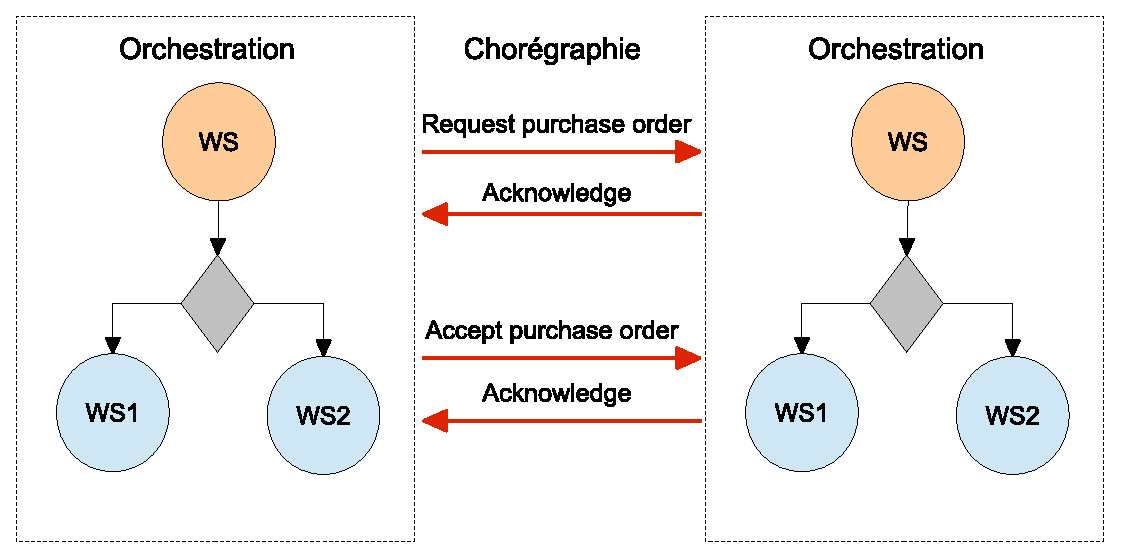
\includegraphics[width=1\textwidth]{figs/orchestration-vs-choregraphie.eps}
    \caption{Orchestration vs Chorégraphie selon Peltz
      \cite{peltz2003web}.}
    \label{fig:orchestration-vs-choregraphie}
\end{figure}

    \subsubsection{Orchestration}
    \label{sec:orchestration}
    Selon Sonia \emph{et al.} \cite{jamal2005environnement}:
    \emph{``L'orchestration des services Web permet de définir
      l'arrangement et l'enchaînement de ces services selon un
      canevas bien défini. Elle décrit la manière par laquelle les
      services peuvent intéragir ensemble tout en incluant l'ordre
      d'exécution des différentes interactions''}.\bigskip

    Barros \emph{et al.} \cite{barros2006standards} définissent
    l'orchestration comme un ensemble de processus exécutés dans un
    ordre prédéfini afin de répondre à un but
    \cite{lopez2008selection}. Ce type de composition se base sur un
    procédé métier exécutable permettant de décrire d'enchaînement et
    les interactions des services basiques collaborant dans une
    composition.\medskip

    L'orchestration offre \textbf{une vision centralisée} de contrôle,
    le procédé est toujours contrôlé par l'un des partenaires
    métiers. Ce dernier joue le rôle d'un chef d'orchestre qui se
    charge d'appeler les services de la composition suivant l'ordre
    d'exécution déjà défini par le processus métier. Le principe de
    l'orchestration est illustré par la figure
    \ref{fig:orchestration}.

    \subsubsection{Chorégraphie}
    \label{sec:choregraphie-sec}
    Selon Sonia \emph{et al.} \cite{jamal2005environnement} : \emph{``
      La chorégraphie permet de tracer la séquence de messages
      échangés dans un contexte de composition des services Web. Elle
      est typiquement liée à la description de conversations
      existantes entre les services tout en impliquant plusieurs
      parties, incluant les clients, les fournisseurs et les
      partenaires''}.\medskip

    D'après Barros \emph{et al.} \cite{barros2006standards}, la
    chorégraphie permet de décrire la composition comme un moyen
    d'atteindre un but commun en utilisant un ensemble de services
    Web. La collaboration entre chaque service Web de la collection
    (faisant partie de la composition) est décrite par des flots de
    contrôle \cite{lopez2008selection}.\medskip

    La chorégraphie offre \textbf{une vision décentralisée} et
    \textbf{globale} du système et exprime une vue d'ensemble des
    services intéragissant dans le cadre d'une composition de
    services. Selon Peltz \cite{peltz2003web}, la chorégraphie
    illustre les différents échanges de messages entre les
    participants. Le principe de la chorégraphie est illustré par la
    figure \ref{fig:choregraphie}.

  \subsection{Stratégies de composition}
  \label{sec:types-de-composition}
  Un modèle de composition de service peut être relativement
  complexe. Il requiert la description et l'organisation de
  l'interaction entre les services et nécessite la gestion de
  plusieurs aspects comme les échanges de données entre les services,
  les pannes ou erreurs éventuelles, le contexte d'interaction, le
  degré d'automatisation des tâches, etc. \medskip

  Il existe une variété de spécifications, de langages et
  d'approches formelles développées dans la littérature concernant la
  composition. Ces techniques sont également classées en fonction de
  différentes dimensions, et selon les travaux effectués dans le champ
  des services web, les définitions des types de composition diffèrent
  d'une communauté à l'autre.\medskip

  Barros \emph{et al.} \cite{barros2006standards} classent la
  composition des services Web en trois catégories : la composition
  comportementale, l'orchestration et la chorégraphie, à l'instar de
  Barros \emph{et al.}, Peltz \cite{peltz2003web} considère que les
  deux dernières \textit{(orchestration, chorégraphie)}.\medskip

  \begin{figure}[h]
    \centering
    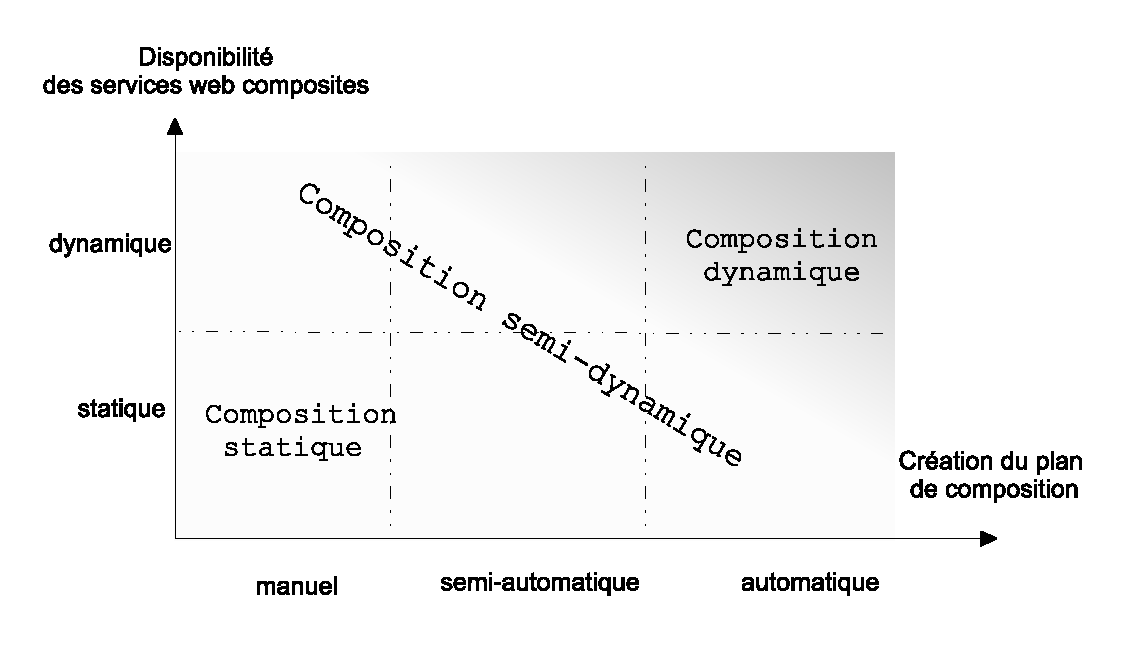
\includegraphics[width=1.1\textwidth]{figs/static-vs-dynamic-composition.eps}
    \caption{Classification des stratégies de composition
      \cite{fluegge2006challenges}.}
    \label{fig:static-vs-dynamic-composition}
\end{figure}
%%% Local Variables: 
%%% mode: latex
%%% TeX-master: "../main"
%%% End: 


  Dans leur analyse de l'état de l'art,
  Fluegge \emph{et al.}\cite{fluegge2006challenges} considèrent l'orchestration et
  la chorégraphie comme des modèles d'exécution appliqués dans le
  contexte d'une composition. Il distingue trois stratégies de
  composition selon la disponibilité des services Web composites lors
  de composition et du degré d'automatisation: composition
  \textbf{statique}, \textbf{semi-dynamique} et \textbf{dynamique}
   comme le montre la figure \ref{fig:static-vs-dynamic-composition}).

    \subsubsection{Composition statique/dynamique}
    \label{sec:comp-stat}
    Selon la disponibilité des services composites, La composition des
    services Web peut être soit une composition statique soit une
    composition dynamique \cite{driss2011approche}:

    \renewcommand{\descriptionlabel}[1]{\hspace{0.5cm}\textbullet~\textsf{#1}}
    \begin{description}
    \item[Composition statique] :est appelée aussi composition
      \textit{Offline} ou pré-compilée. c'est une composition qui
      utilise des services basiques qui sont préalablement définis
      d'une façon figée et qui ne peuvent pas changer en fonction du
      contexte du client. Ce type de composition engendre des
      applications peu flexibles, parfois inappropriées avec les
      exigences des clients.

    \item[Composition dynamique]: appelée aussi composition
      \textit{Online}, post-compilée ou encore réactive. Elle se
      réfère à la sélection des services basiques à la volée. Autrement
      dit, la sélection des services basiques ne peut pas être définie
      à l'avance mais elle sera faite au moment de l'exécution en
      fonction des contraintes imposées par le client. Ceci permet d'
      élaborer différents scénarios de composition qui offrent les
      mêmes fonctionnalités et qui tiennent compte de la dynamique de
      la situation du client.
    \end{description}
    \enddescription

    \subsubsection{Composition manuelle/automatique}
    \label{sec:comp-manu}
    Selon le degré d'automatisation, nous distinguons:

    \renewcommand{\descriptionlabel}[1]{\hspace{0.5cm}\textbullet~\textsf{#1}}
    \begin{description}
    \item[Composition manuelle]: Suppose que l'utilisateur gère la
      composition manuellement et sans l'aide d'outils dédiés.

    \item[Composition semi-automatique]: C'est un pas en avant en
      comparaison avec la composition manuelle, dans le sens qu'elle
      fait des suggestions sémantiques pour aider à la sélection des
      services Web dans le processus de composition.

    \item[Composition automatique]: La composition automatique (ou
      encore dynamique selon \cite{fluegge2006challenges}) permet un
      développement plus rapide des applications à base de
      services. Elle consiste à préciser la requête d'un utilisateur
      sous forme d'objectifs à satisfaire. Un moteur de composition
      \textit{``intelligent''} choisit la combinaison des services
      répondant à l'objectif décrit. Il génère la composition des
      services adéquats de manière transparente à l'utilisateur. Ce
      principe a interpellé plusieurs communautés de recherche
      travaillant dans le domaine de l'intelligence artificielle.
      \cite{elie2010}
    \end{description}
    \enddescription

\section{Langages pour la composition des services Wab}
\label{sec:lang-de-comp}
Afin de supporter la composition des services Web, plusieurs langages
ont été proposés pour décrire et mettre en oeuvre une composition.
Dans cette section nous allons faire un tour d'horizon des principaux
standards et langages.

  \subsection{BPEL}
  \label{sec:bpel}
  \acrshort{bpel} est une spécification du consortium OASIS
  \footnote{\url{https://www.oasis-open.org}} issue de la fusion des
  spécifications \acrshort{xlang} Microsoft et \acrshort{wsfl} d'IBM ,
  il hérite les caractéristiques d'un langage structuré en blocs de
  \textsc{XLANG} ainsi que les caractéristiques d'un graphe direct de
  \acrshort{wsfl} \cite{driss2011approche}.\medskip

  \acrshort{bpel} \textit{(appelé aussi \acrshort{bpel4ws} ou
    \acrshort{ws-bpel})} est le langage d'\textbf{orchestration} le
  plus utilisé dans l'industrie permettant la coordination des
  interactions entre l'instance du service composite et ses
  partenaires sous forme d'un schéma \acrshort{xml} \textit{(le script
    d'orchestration)}, il définit le processus, l'enchaînement et
  l'ordonnancement des actions qui seront exécutées par le moteur
  d'orchestration, agissant comme une machine virtuelle capable
  d'exécuter \textbf{le procédé métier} interprétable de
  \textbf{coordination} \cite{chollet2009orchestration}.\medskip

  \acrshort{bpel} repose sur un modèle constitué d'activités de
  coordination qui peuvent être de deux types: les activités de base
  ou élémentaires comme l'invocation (invoke) d'un service, l'attente
  d'une réponse et la génération d'une réponse (\verb|reply|), et les
  activités composites permettant du contrôle du flot de données comme
  les séquences (\verb|sequence|), les exécutions en parallèle
  (\verb|flow|) et les branchements (\verb|switch|, \verb|if|).

  \subsection{WS-CDL}
  \label{sec:WS-CDL}
  \acrshort{ws-cdl} \footnote{\url{http://www.w3.org/TR/ws-cdl-10/}}
  \cite{kavantzas2005web} est un langage de composition des services de
  type \textbf{chorégraphie} qui permet de décrire une vision
  \textbf{globale} des collaborations entre les services Web
  \cite{elie2010}, à l'instar des standards de services Web,
  \textsc{WS-CDL} est basé sur \textsc{XML}, il complète la
  description \acrshort{wsdl} des services Web afin de décrire les
  points d'interactions entre les services Web engagés dans une
  composition. Contrairement à la spécification \acrshort{bpel}
  \ref{sec:bpel}, Les interactions des services sont décrites d'une
  manière \textit{peer-to-peer}, Il n'y a pas de notion de
  coordination ou d'un service Web principal d'orchestration.\medskip

  \textsc{WS-CDL} reprend et développe la spécification
  \acrshort{wsci} \footnote{\url{http://www.w3.org/TR/wsci/}}
  \cite{arkin2002web} décrivant les séquences ordonnées de messages
  impliquant plusieurs entités (services Web) engagées dans une
  composition visant à accomplir un objectif commun, il permet de
  décrire les règles selon lesquelles une collaboration doit avoir
  lieu par le biais d'un fichier \textsc{XML} décrivant une
  chorégraphie.

  \subsection{WSMF}
  \label{sec:wsmf}
  \acrshort{wsmf} \cite{fensel2002web} est un initiative européen pour
  fournir une plate-forme riche de modélisation décrivant plusieurs
  aspects de services web. Son objectif principale est de permettre le
  commerce électronique (\emph{E-commerce}) par l'application de web
  sémantique aux services Web.  Le standard \acrshort{wsmf} est centré
  autour de deux principes complémentaires \cite{baryannis2010}: un
  découplage fort des différents aspects des applications de
  \textit{E-commerce}, et des mécanismes de médiation permettant un
  dialogue automatique entre les différents composants.\medskip

  \acrshort{wsmf} comprend quatre éléments principaux:

  \SpecialItem
  \begin{itemize}
  \item Des ontologies qui fournissent la terminologie utilisée par
    les autres éléments.

  \item Un répertoire d'objectifs qui définit les problèmes qui
    doivent être résolus par les Web services.

  \item Des descriptions des services Web qui définissent les
    différents aspects liés aux Web services

  \item Des médiateurs qui ont en charge les problèmes
    d'interopérabilité.
  \end{itemize}
  \enddescription

  Il y a deux principaux projets en WSMF : \textsc{SWWS} et
  \acrshort{wsmo}. Le standard \textsc{SWWS} fournit un cadre de
  description, de découverte et de médiation pour les services Web,
  tandis que l'ontologie de service \acrshort{wsmo} inclut des
  définitions pour les objectifs, les médiateurs et les services Web.

  \subsection{OWL-S}
  \label{sec:owl-s}

  \begin{figure}[h]
    \centering
    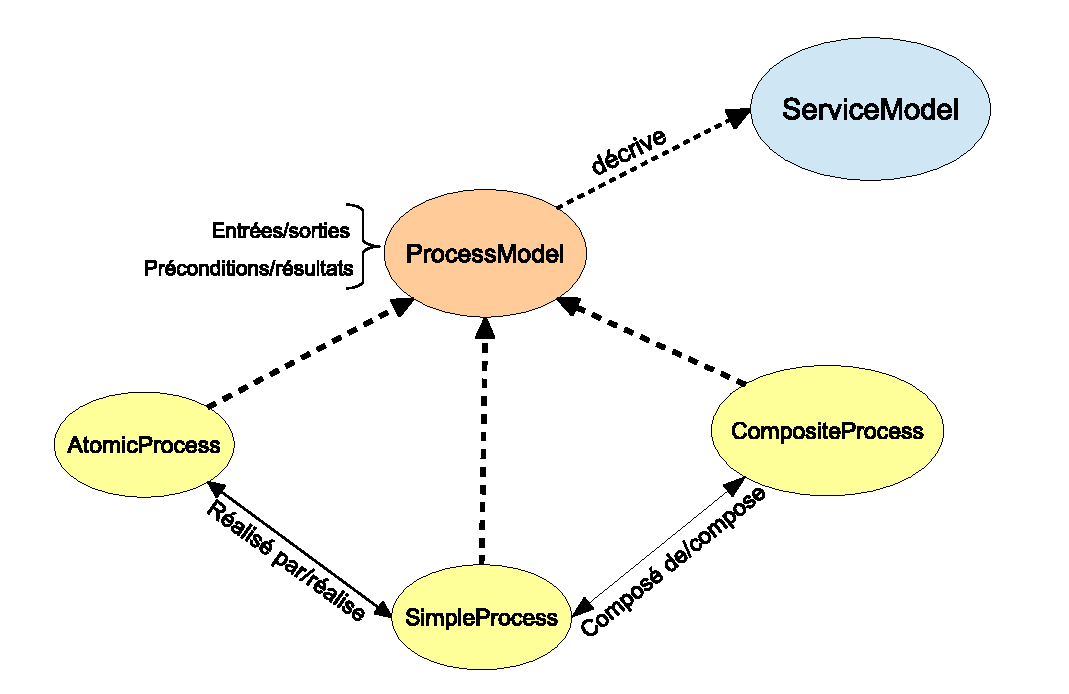
\includegraphics[width=0.95\textwidth]{figs/owls-processModel.eps}
    \caption{Les éléments d'une ontologie ProcessModel}
    \label{fig:owls-processModel}
\end{figure}
%%% Local Variables:
%%% mode: latex
%%% TeX-master: "../main"
%%% End:

  \textsc{OWL-S} définit une sous-classe de \verb|ServiceModel|
  appelée \verb|ProcessModel|, elle est utilisée pour décrire le
  service comme un processus. Le modèle de processus identifie trois
  types de processus schématisés par la figure
  \ref{fig:owls-processModel}:

  \renewcommand{\descriptionlabel}[1]{\hspace{0.5cm}\textbullet~\textsf{#1}}
  \begin{description}
  \item[Le processus atomique]: (\verb|AtomicProcess|) directement
    invoqué par l'intermédiaire d'un \verb|ServiceGrounding|

  \item[Le processus composé]: (\verb|CompositeProcess|) décomposable
    en d'autres processus plus simples en utilisant les commandes de
    contrôle (par exemple: \textit{if/else, sequences} etc.

  \item[Le processus simple]: (\verb|SimpleProcess|) non-invoquable,
    il fournit simplement une vue sur un processus atomique ou une
    représentation simplifié d'un processus composé.
  \end{description}
  \enddescription

  Dans \cite{martin2004owl}, les auteurs discutent les avantages de la
  description de service plus riche soutenue par \textsc{OWL-S}. il
  décrivent comment \textsc{OWL-S} est utilisé dans le contexte d'autres
  standards, tels que \textsc{WSDL}, \textsc{UDDI} et \acrshort{bpel}.

  \subsection{Comparaison}
  \label{sec:langs-comparaison}
  Une composition des services Web nécessite la satisfaction de
  plusieurs exigences techniques \cite{sheng2014web,
    bucchiarone2006survey} , le tableau
  \ref{comparaison-des-standards-et-langages-de-composition} montre une
  comparaison entre les langages et standards présentés dans cette
  section selon les critères suivants:

  \begin{table}[htb!]
  \centering
  \begin{tabular}{|lcccc|}
    \hline
    \head{Langages}& \textsc{BPLE} & \textsc{WS-CDL} & \textsc{WSFM} & \textsc{OWL-S}\\
    \hline\hline
    \textbf{Composabilité} &\verb|+|& \verb|+|&\verb|-|&\verb|+|\\
    \textbf{Representation du rôle} &\verb|+|& \verb|+|&\verb|-|&\verb|-|\\
    \textbf{Support des structures complexes} &\verb|+|& \verb|+|&\verb|-|&\verb|+|\\
    \textbf{Compensabilité} &\verb|+|& \verb|+|&\verb|-|&\verb|-|\\
    \textbf{Support du sémantique} &\verb|-|& \verb|-|&\verb|+|&\verb|+|\\
    % TODO réviser critères
    \textbf{Support industriel} &\verb|+|& \verb|-|&\verb|-|&\verb|+|\\
    \hline
  \end{tabular}
  \newline

  \raggedright
  (\verb|+|) support, (\verb|-|) pas du support.
  \caption{Comparaison des standards et langages de composition}
  \label{comparaison-des-standards-et-langages-d-composition}
\end{table}
%%% Local Variables:
%%% mode: latex
%%% TeX-master: "../main"
%%% End:


  \renewcommand{\descriptionlabel}[1]{\hspace{0.5cm}\textbullet~\textsf{#1}}
  \begin{description}
  \item [La composabilité]: indique la capacité d'assembler des
    services participants dans un processus de composition et de
    modéliser les interactions entre eux.

  \item [La représentation du rôle]: indique la capacité de refléter
    le comportement que le participant doit présenter afin d'intéragir
    avec le processus de composition.

  \item [Le support des structures complexes]: la capacité de
    modéliser les structures complexes qui reflètent les règles des
    actions réalisées dans le processus de composition logique
    d'exécution et de commande.

  \item [Compensabilité]: est la capacité de gérer les exceptions de
    processus lors de l'exécution du processus de composition.

  \item [le support de la sémantique]: est la capacité de représenter la
    sémantique des services participants pour faciliter la découverte
    des services et la composition dynamique.

  \item [le support industriel]: indiqué par la qualité des outils et
    le support industriel de la technologie.
  \end{description}
  \enddescription

  D'après le tableau
  \ref{comparaison-des-standards-et-langages-de-composition}, nous
  pouvons constater que tous les langages sauf \textsc{WSMF}
  supportent la modélisation des structures complexes, seulement
  \acrshort{bpel} et \textsc{WS-CDL} ont le support complet de la
  définition des rôles et la compensation. On peut aussi remarquer que
  seul \textsc{OWL-S} et \textsc{WSMF} permettent la
  composition sémantique des services Web.

  \section{Les approches de composition dynamique des services web}
  \label{sec:comp-dynam}
  Il existe une multitude d'approches de composition des
  services visant à décrire l'interaction entre les services Web afin de 
  construire de nouveaux services composites répondant à un objectif donné. 
  Selon l'approche proposée, les interprétations différent de ce que devraient être
  traitées dans une approche de composition, ils diffèrent également
  sur le degré d'automatisation impliqué dans le processus allant des
  approches semi-automatisées à entièrement automatisés.\medskip

  Dans cette section, nous allons décrire et classifier les approches
  principales de composition proposées par différents auteurs issus
  de plusieurs communautés de recherche. La classification présentée
  par la suite est basée essentiellement sur l'état de l'art fait par
  Baryannis \emph{et al.}\cite{baryannis2010}.
  Nous distinguons quatre catégories de composition dynamique des services Web:

  \renewcommand{\descriptionlabel}[1]{\hspace{0.5cm}\textbullet~\textsf{#1}}
  \begin{description}
  \item[La composition basée sur les workflows]: Ces approches
    exploitent les résultats des recherches dans le domaine des
    \textit{workflows}.

  \item[La composition dirigée par les modèles]: Ces approches
    utilisent les langages de modélisation (les réseaux de Petri,
    \textsc{UML}) pour décrire la composition des services.

  \item[La composition algébrique et mathématique des services web]:
    Ces approches utilisent des méthodes mathématiques (logique
    mathématique, algèbre).

  \item[La composition basée sur les techniques de planification]: Ces
    approches traitent le problème de composition comme un problème de
    planification.
  \end{description}
  \enddescription

  \subsection{La composition  basée sur les workflows}
  \label{sec:les-approches-basees}
  S'appuyant principalement sur le fait qu'un service composite est
  conceptuellement similaire à un \textit{workflow}, il est possible
  d'exploiter les connaissances accumulées dans la communauté de
  \textit{workflow} afin de faciliter la composition des services
  Web. Un \textit{workflow} est un flux d'informations au sein d'une
  organisation, telle que la transmission de documents entre les
  personnes. Il modélise une séquence d'opérations réalisées par
  différentes entités au sein de l'organisation. Pratiquement, un
  \textit{workflow} est considéré comme la modélisation d'un ensemble
  de tâches, accomplies par différents acteurs impliqués dans la
  réalisation d'un processus métier. La modélisation de la composition
  des services sous forme d'un processus métier est de plus en plus
  populaire.\medskip

  Les approches de composition ded services Web basées sur les
  techniques de \textit{workflow} étaient l'une des premières solutions
  proposées pour la composition automatique des services
  Web. Initialement, la plupart des travaux ont porté sur la
  composition statique et manuelle. Cependant, des travaux plus récents
  \cite{majithia2004framework, ardagna2007paws, fujii2006semantics,
    fujii2009semantics} ont tenté de réaliser la composition
  dynamique des services Web. En raison de la popularité de
  \acrshort{bpel} dans le milieu industriel, la plupart des approches
  dans cette catégorie l'emploient d'une manière ou d'une
  autre.\medskip

  Il faut noter que même si les approches
  de composition à base de \textit{workflow} ont évolué afin de
  supporter la composition automatique, les résultats restent limités à
  des schémas de composition simples tels que l'exécution séquentielle
  et parallèle. Cette lacune a été comblée en combinant méthodes à
  base de \textit{workflow} avec des techniques de planification
  issues du domaine d'intelligence artificielle. Ces approches seront
  examinées dans la quatrième catégorie \ref{sec:tech-de-plan}.

  \subsection{La composition dirigée par les modèles}
  \label{sec:model-based-composition}
  L'ingénierie dirigée par les modèles \acrshort{mdo} est une
  méthodologie de développement logiciel où l'accent est mis sur la
  création des modèles abstraits, indépendants de la plateforme et de
  la technologie.
  Un paradigme de modélisation doit fournir des
  modèles logiques du point de vue de l'utilisateur tout en restant
  suffisamment précis pour servir de base à l'implémentation
  \cite{dumez2010approche}. Les approches dans cette catégorie
  utilisent des méthodes déjà explorées et des modèles bien établis
  pour représenter un système de composition afin de pâlir la
  complexité croissante de cette dernière utilisant une description
  plus abstraite au dessus de la description traditionnelle de
  services dans \textsc{WSDL}, \textsc{OWL-S} ou similaire.\medskip

  \textsc{UML} \cite{rumbaugh2004unified} est un langage de
  modélisation maintenu par
  l'\textsc{OMG}\footnote{\url{http://www.omg.org}} qui s'est
  standardisé de par sa position dominante dans l'industrie du
  logiciel. \textsc{UML} est un langage polyvalent permettant de
  modéliser un système selon différents points de vue. Le point de vue
  statique ou structurel du système et le point de vue dynamique
  représente le comportement dynamique d'un système en montrant les
  interactions entre les objets ou les changements d'états au sein
  d'un objet.\medskip

  Skogan \textit{et al.}  \cite{skogan2004web} proposent une méthode
  qui utilise les diagrammes d'activités \textsc{UML} pour modéliser
  la composition des services. Ces diagrammes sont utilisés pour
  générer un processus exécutable d'orchestration \acrshort{bpel}
  utilisant des transformations \textsc{XSLT}, ce travail se limite à
  la description syntaxique des service Web utilisant les documents
  \textsc{WSDL} comme des entrées de la transformation
  \textsc{UML}. Dans \cite{gronmo2005model} les auteurs essayent de
  soulèver cette limitation en considérant également l'enrichissement
  sémantique des services avec des ontologies \textsc{OWLS} et des
  annotations \acrshort{wsmo}.\medskip

  Les réseaux de Petri \cite{petri1962kommunikation} constituent une
  approche bien établie pour la modélisation des processus. Un réseau
  de Petri est un graphe dirigé, connecté et biparti qui représente
  les transitions entre plusieurs états du système, ainsi que les
  ressources disponibles \cite{dumez2010approche}. Hamadi et
  Benatallah dans \cite{hamadi2003petri} proposent une méthode de
  modélisation basée sur les réseaux de Petri pour modéliser le flux
  de contrôle et la sémantique des compositions des services en
  assignant une transition à chaque appel de service et une place à
  chaque état entre les appels. Chaque service composite est modélisé
  par un réseau de Petri contenant un état d'entrée et de sortie
  permettant de modéliser respectivement la réception et l'émission
  d'informations par le service composite. Dans
  \cite{ouyang2007formal}, les auteurs présentent une traduction
  complète de \acrshort{bpel} en réseaux de Petri permettant la
  vérification automatique des processus \acrshort{bpel}.

  \subsection{La composition algébrique et mathématique}
  \label{sec:les-apprc-math}
  Cette catégorie d'approches inclues toutes les approches qui ont la
  caractéristique commune à être fondée sur des bases mathématiques
  telles que la logique temporelle et linéaire, calcul formel, calcul
  algébrique des processus et autres méthodes mathématiques. De
  nombreux langages présentés comme des algèbres de processus, ont
  été développés pour une compréhension formelle de la spécification
  d'applications à services \textsc{SOA}. Les langages d'orchestration
  tels que \acrshort{xlang} et \acrshort{bpel} sont fortement inspirés
  de la métaphore de communication inspirée du $\pi$-calcul basé sur
  l'échange de messages dans un contexte distribué.\medskip

  Les algèbres de processus sont des formalismes de description
  formelle pour la spécification des systèmes logiciels, en particulier
  pour les systèmes concurrentiels \cite{dumez2010approche}. Elles
  fournissent des outils pour la description de haut niveau des
  interactions et des synchronisations entre les processus. Plusieurs
  algèbres de processus ont été décrites, parmi les plus anciennes on
  peut citer \acrshort{csp} présenté par Hoare
  \cite{hoare1978communicating}, \acrshort{ccs} proposé par
  Milner \cite{milner1982finite, milner1989communication} et le
  $\pi$-calcul \cite{milner1992calculus}.\medskip

  Milanovic \textit{et al.} \cite{milanovic2004current} montre que
  l'utilisation des langages algébriques de processus et langages
  formels, comme le \textsc{CCS} et le $\pi$-calcul été préconisée
  pour la composition des services Web, car les spécifications de
  processus comprises dans les standards des services Web comme
  \acrshort{wsmo} ou \acrshort{wsmf} sont formellement fondées sur 
  l'algèbre des processus.\medskip

  La composition algébrique permet de modéliser les services comme des
  processus mobiles pour assurer une vérification de certaines
  propriétés telles que l'exactitude, la sécurité, la vivacité
  \textit{(liveness)}, et la gestion des ressources. La théorie des
  processus mobiles est basée sur le $\pi$-calcul, dans lequel
  l'entité de base est un processus pouvant être un processus vide,
  un choix (branchement) entre plusieurs opérations
  d'\textit{Entrées/Sorties} et leurs continuations, une composition
  parallèle, une définition récursive, ou une invocation récursive
  \cite{zahirathesis2008}.\medskip

  Dans \cite{koshkina2004modelling}, la sémantique du langage de
  chorégraphie \textsc{WS-CDL} est décrite à l'aide de \textsc{CSP}
  pour permettre la vérification automatique de propriétés. Un
  travail similaire est réalisé dans \cite{li2007modeling} où des
  règles sont présentées pour traduire chaque construction syntaxique
  de \textsc{WS-CDL} en \textsc{CSP}.\medskip

  Rao \textit{et al.} \cite{rao2004logic} proposent l'utilisation de
  la logique linéaire pour la composition automatique des services
  Web. La logique linéaire est une extension de la logique classique
  du premier ordre pour modéliser la notion d'évolution d'états. Les
  auteurs proposent une méthode de traduction automatique des
  descriptions \textsc{OWL-S} à des axiomes de la logique
  linéaire. Ensuite, ils utilisent la démonstration automatique des
  théorèmes pour produire des schémas abstraits de composition, qui
  sont ensuite transformés à des modèles de \textit{workflows}
  \acrshort{bpel} en utilisant un langage d'algèbre des processus
  inspiré par le $\pi$-calcul.\medskip

  \subsection{La composition basée sur les techniques de
    planification}
  \label{sec:tech-de-plan}
  Cette catégorie d'approches de composition dynamique des services Web
  encadre tous les efforts de recherche qui utilisent des techniques
  de planification en intelligence artificielle \textit{(AI)} afin de
  générer un schéma de composition. Les techniques de planification en
  \textit{AI} impliquent la génération d'un plan contenant une suite
  d'actions qui mènent à un état final à partir d'un état
  initial. Toutes les approches de cette famille reposent sur l'une
  des nombreuses techniques de planification que la communauté
  \textit{AI} a proposée et les utilisent dans le cadre de la
  composition des services Web.\medskip

  Un problème de planification peut être décrit comme un
  \textit{quintuple } \textit{$\{S, s_0,G, A, \Gamma\}$}
  \cite{carman2003web}, où $S$ est un ensemble fini ou énumérable
  d'états possibles du système considéré, $s_0\subset S$ désigne
  l'état initial du système, $G\subset S$ désigne l'ensemble des états
  buts que système de planification tente d'atteindre, $A$ est
  l'ensemble des actions possibles qui peuvent être effectuées afin
  d'atteindre l'état but.  \textit{$\Gamma \subset S \times A \times
    S$} est une relation de transition qui décrit l'état résultant
  quand une action particulière est exécutée dans un état donné
  $S$. Si nous considérons $A$ comme l'ensemble des services
  disponibles , $G$ soit le service requis par le client, et un modèle
  d'état liée à $S$ , $s_0$ et $\Gamma$ et appliquée sur les services
  disponibles, nous pouvons utiliser des solutions existantes pour la
  planification en \textit{AI} afin de résoudre le problème de
  composition des service Web. Il est à noter que cette corrélation ne
  soit pas suivie par toutes les approches de cette
  catégorie.\medskip

  Les approches de composition basées sur les techniques de
  planification peuvent se catégoriser en quatre grands familles
  \cite{baryannis2010}:

  \renewcommand{\descriptionlabel}[1]{\hspace{0.5cm}\textbullet~\textsf{#1}}
  \begin{description}
  \item [La planification classique:] Les approches de planification
    classique \cite{akkiraju2004executing, zeng2008dynamic} peuvent
    être regroupées en deux familles: Les approches qui
    utilisent les algorithmes de planification dans un espace d'états
    \textit{(state space planning)} qui sont les plus simples, et celles
    qui utilisent la planification dans un espace de plans \textit{(plan space planning)}.

  \item [La planification néoclassique:] Ces approches regroupent des
    techniques qui étendent la notion classique de
    planification. Celles-ci comprennent la planification basée sur les
    graphes \ref{sec:graph-base-composition}, le problème de la
    satisfaction de contraintes \textit{(CSP)}
    \cite{paik2007automatic} et la planification à base de règles
    \textit{(rules-based calculus)} \cite{medjahed2004semantic,
      rao2006mixed}.

  \item [Heuristiques et stratégies de contrôle:] Ces approches
    comportent la planification hiérarchique \cite{wu2003automating,
      sirin2004htn}, planification d'ordre partiel \cite{peer2005pop,
      klusch2005semantic}, et la planification basée sur le calcul
    situationnel \cite{mcilraith2002adapting, sohrabi2009web}.

  \item [Autres techniques de planification:] Dans cette famille nous
    pouvons citer les approches basées sur le calcul des évènements
    \cite{aydin2008automated} et la planification basée sur le
    \textit{model checking}
    \cite{pistore2004planning,pistore2005automated}.
  \end{description}
  \enddescription

  \section{Les approches de composition basée sur le modèle graphe}
  \label{sec:graph-base-composition}

  La découverte d'un service composite à partir d'un graphe de
  dépendance consiste à trouver le meilleur chemin dans le graphe qui
  génère les sorties exprimées dans la requête. La recherche peut se
  baser sur l'optimisation d'une fonction d'utilité qui tient compte
  du degré de \textit{Matching} entre les services et aussi de la qualité de
  service qui peut être fournie par les services concrets. A cet
  effet, les méthodes de recherche du meilleur chemin de la théorie
  des graphes peuvent être exploitées.  Les méthodes de composition
  utilisant le modèle de graphe peuvent être classées en deux
  catégories selon que le graphe de dépendance soit construit à priori
  (en phase de publication des services) ou pendant le traitement de
  la requête de composition.

  \newpage
  \subsection{Génération Online du graphe de dépendance}
  \label{sec:generation-online}
  Étant donnée une requête d'utilisateur, les services candidats à
  la composition sont découverts et interconnectés au moment du
  traitement de la requête (dynamiquement). Le graphe généré
  contient un nombre restreints de services candidats mais peut
  inclure plusieurs alternatives de plans possibles. Le plan de
  composition sera dérivé du graphe généré en optimisant la qualité du
  plan (degré de \textit{Matching}, les paramètres
  \textit{non-fonctionnels}).\bigskip

  Dans \cite{liang2005and}, Liang \textit{et al.} présentent une
  formalisation du problème de composition des services comme un
  problème de recherche dans un graphe \textit{And/Or}. Suite à une
  requête dans un domaine spécifique choisi par le client, un graphe
  de composition \textit{SGD} (\textit{Service dependecy graph}) est
  construit dynamiquement reflétant les dépendances fonctionnelles
  entre les services du domaine.\medskip

  Le graphe généré contient des nœuds et des connecteurs de deux
  types: des connecteurs \textit{And} et des connecteurs
  \textit{Or}. Un connecteur \textit{And} relie des services avec un
  autre s'il existe une relation de type \textit{And} entre
  les paramètres de ces services. Donc, toutes les entrées fournies par
  les services doivent être disponibles pour l'exécution du service
  destinataire. Des services sont connectés par un \textit{Or} avec un
  autre service s'il existe une relation logique de type \textit{Or}
  entre les paramètres des ces services. Donc, n'importe quel service
  pourra produire l'entrée requise par le service
  destinataire.\medskip

  L'algorithme de recherche est appliqué itérativement pour trouver le
  service composite minimal et complet satisfaisant la requête puis
  soumis à évaluation par l'utilisateur jusqu'à ce qu'il valide le
  résultat.\bigskip

  Dans \cite{lecue2006formal}, Freddy et Léger présentent un modèle
  formel pour effectuer la composition automatique des services Web par
  le biais de liens causals. Les auteurs introduisent la notion de
  \textit{``Causal link matrix''}, Cette matrice est nécessaire comme
  point de départ pour appliquer des approches de recherche basées sur
  la régression (ou progression), le modèle prend en charge un
  contexte sémantique afin de trouver des plans correctes et complets
  comme solutions au problème de composition des service Web.\bigskip

  Dans \cite{omer2009dependency}, les auteurs supposent que les
  services candidates avaient été déjà découverts localement par un
  algorithme de découverte orienté but. L'exécution du plan se déroule
  en quatre principales étapes:

  \SpecialItem
  \begin{itemize}
  \item La première est la génération du graphe de dépendance grâce à
    un algorithme qui utilise une matrice d'adjacence des dépendances
    \textit{Inputs/Outputs} entre les services. Les dépendances sont
    identifiées si au moins une paire de paramètres (des
    \textit{Input($WS_1$)} et \textit{Output($WS_2$)}) est en
    relation \textit{exact} ou \textit{plug-in} selon
    \cite{paolucci2002semantic}.

  \item Extraction du graphe des dépendances cyclique (en boucle) en
    utilisant l'algorithme \cite{tarjan1973enumeration}.

  \item Régénération d'un nouveau graphe des dépendances acyclique en
    remplaçant chaque sous-graphe cyclique par un nœud composé.

  \item l'extraction du plan de composition et la génération du plan
    final; les nœuds composés seront remplacés par leurs sous-plans
    respectifs.\medskip
  \end{itemize}
  \enddescription

  La principale contribution de ce travail est la manière de traiter
  les cas de boucle dans un graphe, ce problème particulièrement a été
  très peu abordé dans ce domaine.\bigskip

  Mahmoud \emph{el al.} \cite{mahmoud2013towards} proposent une
  approche de composition automatique des services à l'aide de graphes
  orientés. Le graphe de composition décrit les liens de dépendance
  entres les services Web, ainsi que leur ordre d'exécution. La requête
  du client définie par un ensemble de paramètres
  d'\textit{entrée/sortie} peut être vue comme un graphe orienté
  composé de services Web. les auteurs modélisent un service Web comme
  une fonction \textit{WS(Parameters, State-of-the-world)}, ou les
  paramètres sont les \textit{entrées/sorties}, et le
  \textit{State-of-the-world} est les conditions préalables et effets
  conditionnels sur le monde.

  \subsection{Génération Offline du graphe des dépendances}
  \label{sec:generation-offline}
  Certains auteurs considèrent qu'il serait plus intéressant
  d'utiliser des informations complètes sur tous les services publiés
  pour assurer une recherche plus exhaustive des services candidats à
  la composition. Pour cela, le graphe de dépendance est pré-généré à
  partir du registre ou sont publiés les services. Par conséquent, le
  graphe inclut toutes les dépendances possibles entre les services
  disponibles, par contre il peut être volumineux et doit être mis à
  jour au fur et à mesure en prévision de certains changements (l'arrivée ou non
  disponibilité des services).\bigskip

  Arpinar \textit{et al.} \cite{arpinar2005ontology} proposent une
  approche semi-automatique permettant la découverte et la composition
  des services Web. L'approche proposée utilise des descriptions et un
  processus ontologique (utilisant l'ontologie \textit{DAML-S}) pour
  découvrir et composer les services dont la sémantique s'aligne avec
  les exigences des utilisateurs. La solution proposée se base sur la
  programmation dynamique en utilisant l'algorithme de
  \textit{Bellman-Ford} pour la recherche du plus court chemin en
  optimisant le temps d'exécution et le degré de similarité sémantique
  entre les services Web.\bigskip

  Dans \cite{gu2008automatic}, Gu Zhifeng \textit{et al.} reprennent
  le travail de \cite{liang2005and} et proposent une version améliorée
  de \textit{SDG} (à savoir \textit{SDG+}). \textit{SDG+} renforce le
  modèle \textit{SDG} avec une déclaration explicite de dépendances
  entre les services candidats via des segments \acrshort{xml}. Les
  auteurs éliminent l'évaluation manuelle requise par l'approche de
  \cite{liang2005and} et présentent une approche automatique de
  composition en appliquant l'algorithme de recherche basé sur
  \textit{SGD} avec quelques modifications.\bigskip

  Hashemian \textit{et al.} \cite{hashemian2006graph} stockent les
  dépendances entres les \textit{(entrées/sorties)} des services
  disponibles dans un graphe dont les sommets représentent les
  paramètres \textit{(entrées/sorties)} et les arcs représentent les
  services. Les auteurs introduisent aussi une algèbre des processus
  pour spécifier le comportement des services Web composites basé sur
  le comportement des plus simples, les structures de composition
  considérées dans ce travail sont les séquences, les branchements
  conditionnels, structures parallèles et la synchronisation.

  Suite à une requête, le processus de composition se déroulera en
  deux étapes:

  \SpecialItem
  \begin{itemize}
  \item Trouver les services potentiels pouvant participer dans la
    composition en cherchant les sous graphes couvrant tous les
    $sommets_{entrées}$ et $sommets_{sorties}$ (fournis dans la
    requête) en utilisant une recherche en largeur d'abords
    (\textit{breath first search}).

  \item La deuxième étape consiste à extraire les plans d'exécution 
    à partir des services découverts.\bigskip
  \end{itemize}

  Talantikite \textit{et al.} \cite{talantikite2009semantic} utilisent
  un \emph{``réseau sémantique des services Web''} décrit en
  \textsc{OWL-S} pour modéliser le graphe des dépendances, ce dernier
  est construit avant toute requête soumise par l'utilisateur. Avec
  une seule itération, l'algorithme de composition sélectionne un plan
  optimale en optimisant la qualité du service composite en terme de
  similarité sémantique, temps de réponse, et espace mémoire.
  Cette technique tire profit des algorithmes de chaînage du
  système expert et les annotations sémantiques.\bigskip

  Dans \cite{elmaghraoui2011graph}, les auteurs modélisent à priori
  toutes les dépendances entre les services dans un graphe de
  composition et aussi sauvegarde tous les meilleurs chemins entre les
  nœuds du graphe dans une matrice en appliquant un algorithme basé
  sur l'algorithme de \textit{Floyd-Warshall}, en optimisant le degré
  du \textit{Matching} sémantique, temps d'exécution, le coût, et la
  disponibilité du service.

  \subsection{Autres travaux basés sur le graphe \textit{Matching}}
  \label{sec:autres-travaux}
  Samuel et \textit{et al.} \cite{samuel2011approach} présentent une
  technique de composition basée sur un graphe de planification
  hiérarchique (\textit{layered}) et pondéré reflétant toutes
  dépendances fonctionnelles possibles entres les services
  disponibles. Les auteurs ont conçu le problème de la composition
  comme un problème de génération de \textit{sorties} requises à partir
  d'un ensemble d'\textit{entrées}. Un nœud de graphe représente
  soit une collection de propositions
  (\textit{pré-conditions/effets}), ou un ensemble des actions
  (services Web). Une arête connecte un niveau de graphe à l'autre.
  Après la construction du graphe de planification, un plan optimal
  de composition est généré en optimisant le temps de réponse, le
  coût, la disponibilité et la fiabilité du service composite.\bigskip

  Cuzzocrea \emph{el al.} \cite{cuzzocrea2011flexible} modélise le
  service composite décrit dans \textit{OWL-S} \textit{Process-Model}
  sous forme d'un graphe orienté (modélise le flux de données et
  structure de contrôle) puis il fait le \textit{matching} à deux
  niveaux avec la requête de l'utilisateur (suppose aussi que la
  requête fournit également le schéma de composition):

  \SpecialItem
  \begin{itemize}
  \item \textit{Matching} des \textit{entrées/sorties} de la requête à
    celle du service composite.

  \item \textit{Matching} de la structure du service décrit dans la
    requête avec celle du service composite publié (la requête est
    aussi décrite sous forme de graphe).
  \end{itemize}
  \enddescription

  \subsection{Discussion et comparaison}
  \label{sec:discussion-comparaison}
  Dans les sections \ref{sec:generation-online},
  \ref{sec:generation-offline} et \ref{sec:autres-travaux}, nous avons
  identifiés les différantes approches pour la composition des services
  Web qui utilisent un modèle graphe pour gérer les dépendances
  fonctionnelles entres les services Web référencés dans un
  annuaire. Ces méthodes sont classées en deux catégories selon que le
  graphe de dépendance soit construit à priori (en phase de
  publication des services) ou pendant le traitement de la requête de
  composition. Le tableau \ref{tab:comparaison-graph-composition}
  récapitule les approches présentées dans ces sections . \bigskip

  Dans une approche \textbf{\textit{Online}}, le graphe est généré de
  manière entièrement dynamique après chaque requête et dont la taille
  ne pose aucun problème. Cependant, cette approche révèle certaine limites:
  
  \SpecialItem
  \begin{itemize}
  \item La majorité des approches \textit{Online} effectuent d'abord une
    phase de découverte des services qui peuvent être candidats à la
    composition. Cependant, le mécanisme de découverte ne tient pas
    compte de la relation de dépendance entre les services. Par
    conséquent, de bons services candidats peuvent être négligés.

  \item Requiert un temps de réponse important qui inclut le temps de
    découverte des services candidats, temps de construction du graphe
    de dépendance et le temps de recherche du plan dans le graphe.

  \item Le passage à l'échelle n'est pas garanti: quand le registre
    devient très important le temps de réponse devient très
    lent.\bigskip

  \end{itemize}
  \enddescription

  Dans l'approche \textbf{\textit{Offline}}, le graphe est construit une
  seule fois puis mis à jour à chaque modification dans le registre
  \acrshort{uddi}. Donc le temps de réponse dépend uniquement de
  l'algorithme de recherche du plan. Par contre, ces approches
  demeurent insuffisantes vis-à-vis de:\medskip

  \SpecialItem
  \begin{itemize}
  \item [Du problème de passage à l'échelle]: En effet les graphes
    générés sont supposés être volumineux ce qui pose un problème
    d'espace de stockage.

  \item [Dynamicité de l'environnement]: des mises à jours fréquentes
    doivent avoir lieu sur le graphe des dépendances ce qui implique un
    coût de maintenance important.\bigskip

  \end{itemize}
  \enddescription

\newpage
\begin{table}[htb!]
  \centering
  \resizebox{1.05\textwidth}{!}{%
    \begin{tabular}{|>{\centering\arraybackslash}m{1.5in}|>{\centering\arraybackslash}m{0.9in}|
        >{\centering\arraybackslash}m{1.6in}|>{\centering\arraybackslash}m{1in}|>{\centering\arraybackslash}m{1.4in}|@{}m{0pt}@{}}
      \hline
      \textbf{Approche}  & \textbf{Génération du graph} & \textbf{Algorithme utilsé}& \textbf{Sémantique} &  \textbf{Les paramètres non-fonctionnels} &\\
      \hline\hline %--------------------------------------------------------------------------------------------------
      % ---------------------------------------------------------------------------------------------------------------
      Liang \textit{et al.} \cite{liang2005and} & Online & Recherche dans un And/Or graph & Non & Non &\\ [6ex] %done
      \hline %\item ------------------------------------------------------------------------------------------------------
      Arpinar \textit{et al.} \cite{arpinar2005ontology}& Offline&Bellman-Ford& Oui & temps d'exécution &\\ [6ex] %done
      \hline %--------------------------------------------------------------------------------------------------------
      Freddy et Léger \cite{lecue2006formal} & Online &  &  &  &\\  [6ex]
      \hline %--------------------------------------------------------------------------------------------------------
      Hashemian \textit{et al.} \cite{hashemian2006graph} & Offline & Recherche en largeur d'abord (BFS) ou en profondeur (DFS) & Oui & Non&\\[12ex] %done
      \hline %-------------------------------------------------------------------------------------------------------
      Gu Zhifeng \textit{et al.} \cite{gu2008automatic}& Offline & Extension de And/Or graph utilisée par \cite{liang2005and}  & Non & Non &\\[12ex]
      \hline %--------------------------------------------------------------------------------------------------------
      Abrehet et Schill \cite{omer2009dependency}& Online & Variation d'une recherche topologique basée sur \cite{ma2007systematic}& Oui & Non &\\[12ex] %done
      \hline %--------------------------------------------------------------------------------------------------------
      Elmaghraoui \textit{et al.} \cite{elmaghraoui2011graph}& Offline & Extension de Floyd-Warshall & Oui & Coût, temps d'exécution, disponiblité.&\\[12ex] % done
      \hline %--------------------------------------------------------------------------------------------------------
      Samuel et Sasipraba \textit{et al.} \cite{samuel2011approach}& TODO & TODO & TODO & TODO&\\[10ex]
      \hline %--------------------------------------------------------------------------------------------------------
      Chaker Ben Mahmoud \textit{et al.} \cite{mahmoud2013towards} &Online & Non définie & Oui & Non &\\[6ex] %done
      \hline %--------------------------------------------------------------------------------------------------------
    \end{tabular}}
  \newline
  \caption{Comparaison des approches de composition basées sur le modèle graph}
  \label{comparaison-graph-composition}
\end{table}
%%% Local Variables:
%%% mode: latex
%%% TeX-master: "../main"
%%% End:

\newpage


Selon notre étude comparative, nous avons pu constater que la deuxième
approche semble plus intéressante car le temps de réponse est beaucoup
meilleur et aussi la découverte est basée sur une vue complète des
relations de dépendance qui pourraient exister entre les services.
Cependant, il faudrait penser à résoudre les problèmes de scalabilité
(passage à l'échelle) et aussi la maintenance du graphe des dépendances
vu le caractère dynamique de l'environnement des services web.  Pour
cette raison, nous avons pensé à utiliser une base de données graphe
pour héberger le graphe des dépendances.

\section*{Conclusion}
\label{sec:conclusion}
\addcontentsline{toc}{section}{Conclusion} \markboth{CONCLUSION}{}

La composition des services constitue une étape primordiale pour
l'automatisation du cycle de vie des services au sein d'une
architecture \acrshort{soa}. Beaucoup d'efforts académiques et
standards industriels ont été émergés afin de permettre une
composition utilisable, correcte et efficace des services Web.\medskip

Dans ce chapitre, nous avons présenté une étude bibliographique des
différentes approches pour la composition des services Web, tout en
mettant l'accent sur les approches automatiques qui exploitent
l'enrichissement sémantique des descriptions de services Web. Dans la
dernière section \ref{sec:graph-base-composition} nous nous sommes
concentrés sur les méthodes qui modélisent le problème de composition
sous forme d'un graphe de planification en distinguant deux approches
principales, d'une part, nous avons les méthodes qui construisent le
graphe de dépendance lors du traitement d'une requête cliente
(\textit{Online}), et d'autre part, on a les méthodes qui stockent au
préalable toutes le dépendances fonctionnelles possibles entre les
services dans un graphe à partir d'un annuaire ou un registre
(\textit{Offline}). Le problème majeur qui se posera dans la deuxième
approche est le passage à l'échelle ou la \textit{scalabilité} du
système vu le caractère dynamique de l'environnement des services web
et le risque d'avoir des services non accessibles dans le schéma de
composition lors du déploiement et l'exécution du service
composite.\medskip

Dans le chapitre suivant, nous nous focalisons sur la présentation des
différents systèmes de gestion des bases de données graphes, que nous
utilisons dans notre approche pour la mise en œuvre d'une composition
dynamique des services Web.

%%% Local Variables:
%%% mode: latex
%%% TeX-master: "../main"
%%% End:
